\documentclass[journal,12pt,twocolumn]{IEEEtran}

\usepackage{setspace}
\usepackage{gensymb}
\singlespacing
\usepackage[cmex10]{amsmath}

\usepackage{amsthm}

\usepackage{mathrsfs}
\usepackage{txfonts}
\usepackage{stfloats}
\usepackage{bm}
\usepackage{cite}
\usepackage{cases}
\usepackage{subfig}

\usepackage{longtable}
\usepackage{multirow}

\usepackage{enumitem}
\usepackage{mathtools}
\usepackage{steinmetz}
\usepackage{tikz}
\usepackage{circuitikz}
\usepackage{verbatim}
\usepackage{tfrupee}
\usepackage[breaklinks=true]{hyperref}
\usepackage{graphicx}
\usepackage{tkz-euclide}

\usetikzlibrary{calc,math}
\usepackage{listings}
    \usepackage{color}                                            %%
    \usepackage{array}                                            %%
    \usepackage{longtable}                                        %%
    \usepackage{calc}                                             %%
    \usepackage{multirow}                                         %%
    \usepackage{hhline}                                           %%
    \usepackage{ifthen}                                           %%
    \usepackage{lscape}     
\usepackage{multicol}
\usepackage{chngcntr}

\DeclareMathOperator*{\Res}{Res}

\renewcommand\thesection{\arabic{section}}
\renewcommand\thesubsection{\thesection.\arabic{subsection}}
\renewcommand\thesubsubsection{\thesubsection.\arabic{subsubsection}}

\renewcommand\thesectiondis{\arabic{section}}
\renewcommand\thesubsectiondis{\thesectiondis.\arabic{subsection}}
\renewcommand\thesubsubsectiondis{\thesubsectiondis.\arabic{subsubsection}}


\hyphenation{op-tical net-works semi-conduc-tor}
\def\inputGnumericTable{}                                 %%

\lstset{
%language=C,
frame=single, 
breaklines=true,
columns=fullflexible
}
\begin{document}

\newcommand{\BEQA}{\begin{eqnarray}}
\newcommand{\EEQA}{\end{eqnarray}}
\newcommand{\define}{\stackrel{\triangle}{=}}
\bibliographystyle{IEEEtran}
\raggedbottom
\setlength{\parindent}{0pt}
\providecommand{\mbf}{\mathbf}
\providecommand{\pr}[1]{\ensuremath{\Pr\left(#1\right)}}
\providecommand{\qfunc}[1]{\ensuremath{Q\left(#1\right)}}
\providecommand{\sbrak}[1]{\ensuremath{{}\left[#1\right]}}
\providecommand{\lsbrak}[1]{\ensuremath{{}\left[#1\right.}}
\providecommand{\rsbrak}[1]{\ensuremath{{}\left.#1\right]}}
\providecommand{\brak}[1]{\ensuremath{\left(#1\right)}}
\providecommand{\lbrak}[1]{\ensuremath{\left(#1\right.}}
\providecommand{\rbrak}[1]{\ensuremath{\left.#1\right)}}
\providecommand{\cbrak}[1]{\ensuremath{\left\{#1\right\}}}
\providecommand{\lcbrak}[1]{\ensuremath{\left\{#1\right.}}
\providecommand{\rcbrak}[1]{\ensuremath{\left.#1\right\}}}
\theoremstyle{remark}
\newtheorem{rem}{Remark}
\newcommand{\sgn}{\mathop{\mathrm{sgn}}}
\providecommand{\abs}[1]{\vert#1\vert}
\providecommand{\res}[1]{\Res\displaylimits_{#1}} 
\providecommand{\norm}[1]{\lVert#1\rVert}
%\providecommand{\norm}[1]{\lVert#1\rVert}
\providecommand{\mtx}[1]{\mathbf{#1}}
\providecommand{\mean}[1]{E[ #1 ]}
\providecommand{\fourier}{\overset{\mathcal{F}}{ \rightleftharpoons}}
%\providecommand{\hilbert}{\overset{\mathcal{H}}{ \rightleftharpoons}}
\providecommand{\system}{\overset{\mathcal{H}}{ \longleftrightarrow}}
	%\newcommand{\solution}[2]{\textbf{Solution:}{#1}}
\newcommand{\solution}{\noindent \textbf{Solution: }}
\newcommand{\cosec}{\,\text{cosec}\,}
\providecommand{\dec}[2]{\ensuremath{\overset{#1}{\underset{#2}{\gtrless}}}}
\newcommand{\myvec}[1]{\ensuremath{\begin{pmatrix}#1\end{pmatrix}}}
\newcommand{\mydet}[1]{\ensuremath{\begin{vmatrix}#1\end{vmatrix}}}
\numberwithin{equation}{subsection}
\makeatletter
\@addtoreset{figure}{problem}
\makeatother
\let\StandardTheFigure\thefigure
\let\vec\mathbf
\renewcommand{\thefigure}{\theproblem}
\def\putbox#1#2#3{\makebox[0in][l]{\makebox[#1][l]{}\raisebox{\baselineskip}[0in][0in]{\raisebox{#2}[0in][0in]{#3}}}}
     \def\rightbox#1{\makebox[0in][r]{#1}}
     \def\centbox#1{\makebox[0in]{#1}}
     \def\topbox#1{\raisebox{-\baselineskip}[0in][0in]{#1}}
     \def\midbox#1{\raisebox{-0.5\baselineskip}[0in][0in]{#1}}
\vspace{3cm}
\title{Assignment 2}
\author{Digjoy Nandi - AI20BTECH11007}
\maketitle
\newpage
\bigskip
\renewcommand{\thefigure}{\theenumi}
\renewcommand{\thetable}{\theenumi}
Download all python codes from 
\begin{lstlisting}
https://github.com/Digjoy12/Signal-Processing/tree/main/Assignment_2/Code
\end{lstlisting}
%
and latex codes from 
%
\begin{lstlisting}
https://github.com/Digjoy12/Signal-Processing/blob/main/Assignment_2/main.tex
\end{lstlisting}
\section*{\textbf{Problem}}
\textbf{(Matrix - Q2.60)} Find the matrix $\vec{X}$ so that 
$$\vec{X}\myvec{1 & 2 & 3\\ 4 & 5 & 6} = \myvec{-7 & -8 & -9\\ 2 & 4 &6}$$
\section*{\textbf{Solution}}
Let,
\begin{align}
    \vec{A} &= \myvec{1 & 2 & 3\\ 4 & 5 & 6}\\
    \vec{B} &= \myvec{-7 & -8 & -9\\ 2 & 4 & 6}
\end{align}
Now, multiplying $\vec{A}^\top$ on both sides,
\begin{align}
    \vec{X}\vec{A}\vec{A}^\top &= \vec{B}\vec{A}^\top\\
   \implies \vec{X} &= \vec{B}\vec{A}^\top(\vec{A}\vec{A}^\top)^{-1}
\end{align}
Therefore,
\begin{align}
    \vec{X} &= \myvec{-7 & -8 & -9\\ 2 & 4 & 6} \myvec{1 & 4\\2 & 5\\3 & 6}(\vec{A}\vec{A}^\top)^{-1}\\
            &= \myvec{-50 & -122\\ 28 & 64} \left[\myvec{1 & 2 & 3\\ 4 & 5 & 6} \myvec{1 & 4\\2 & 5\\3 & 6}\right]^{-1}\\
            &= \myvec{-50 & -122\\ 28 & 64}\left[\myvec{14 & 32\\32 & 77}\right]^{-1}\\
            &= \myvec{-50 & -122\\ 28 & 64}\myvec{\cfrac{77}{54}&\cfrac{-16}{27}\\ \cfrac{-16}{27}& \cfrac{7}{27}}\\
            &= \myvec{1 & -2\\2 & 0}
\end{align}
\textit{Alternate Solution:-}\\
Given,
\begin{align}
    \vec{X}\myvec{1 & 2 & 3\\ 4 & 5 & 6}_{2 \times 3} = \myvec{-7 & -8 & -9\\ 2 & 4 &6}_{2 \times 3}\label{0.0.1}
\end{align}\\
Therefore,
$\vec{X}$ is a $2 \times 2$ matrix.\\
Let,
\begin{align}
\vec{X} = \myvec{a & b \\ c & d}    
\end{align}
Now our equation \eqref{0.0.1} becomes, 
\begin{align}
  \myvec{a & b \\ c & d} \myvec{1 & 2 & 3\\ 4 & 5 & 6} &= \myvec{-7 & -8 & -9\\ 2 & 4 &  6} \\
  \implies \myvec{a+4b & 2a+5b & 3a+6b\\ c+4d & 2c+5d & 3c+6d} &= \myvec{-7 & -8 & -9\\ 2 & 4 &6} 
\end{align}\\
Since, the matrices are equal, therefore the corresponding elements are equal too.
\begin{align}
    a + 4b &= -7 \label{0.0.5}\\
    2a + 5b &= -8 \label{0.0.6}\\
    3a + 6b &= -9\\
    c + 4d &= 2 \label{0.0.8}\\
    2c + 5d &= 4 \label{0.0.9}\\
    3c + 6d &= 6
\end{align}\\
Now, \eqref{0.0.5} and \eqref{0.0.6} are two equation with a and b variables, which can be expressed in vector form as 
\begin{align}
    \myvec{1 & 4 \\ 2 & 5}\myvec{a \\ b} &= \myvec{-7 \\ -8}
\end{align}\\
The corresponding augmented matrix is
\begin{align}
    	\myvec{
		1 & 4 & \vrule & -7 \\
		2 & 5 & \vrule & -8 \\
	}
\end{align}\\
We use the Guass Jordan Elimination method as:
\begin{align}
	\myvec{
		1 & 4 & \vrule & -7 \\
		2 & 5 & \vrule & -8 \\
	}
	\\
	\xleftrightarrow[]{R_2 \rightarrow R_2 - 2R_1}
	\myvec{
		1 & 4 & \vrule & -7 \\
		0 & -3 & \vrule & 6 \\
	}
	\\
	\xleftrightarrow[]{R_2\rightarrow \frac{-1}{3}R_2}
	\myvec{
		1 & 4 & \vrule & -7 \\
		0 & 1 & \vrule & -2 \\
	}
	\\
	\xleftrightarrow[]{R_1 \rightarrow R_1 - 4R_2}
	\myvec{
		1 & 0 & \vrule & 1 \\
		0 & 1 & \vrule & -2 \\
	}
\end{align}\\
Therefore, the values of $a$ and $b$ are:
\begin{align}
	a &= 1 \\
	b & = -2
\end{align}\\
\begin{figure}[!h]
\centering
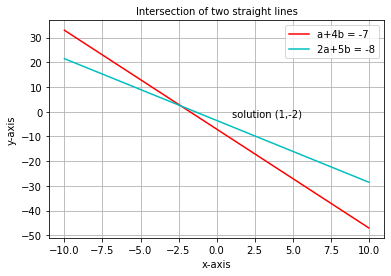
\includegraphics[width=\columnwidth]{plot1.png}
\caption{Plot of the lines}
\label{plt_1}
\end{figure}

Now, \eqref{0.0.5} and \eqref{0.0.6} are two equation with c and d variables, which can be expressed in vector form as 
\begin{align}
  \myvec{1 & 4 \\ 2 & 5}\myvec{c \\ d} &= \myvec{2 \\ 4} 
\end{align}
The corresponding augmented matrix is
\begin{align}
    	\myvec{
		1 & 4 & \vrule & 2 \\
		2 & 5 & \vrule & 4 \\
	}
\end{align}\\
We use the Guass Jordan Elimination method as:
\begin{align}
	\myvec{
		1 & 4 & \vrule & 2 \\
		2 & 5 & \vrule & 4 \\
	}
	\\
	\xleftrightarrow[]{R_2 \rightarrow R_2 - 2R_1}
	\myvec{
		1 & 4 & \vrule & 2 \\
		0 & -3 & \vrule & 0 \\
	}
	\\
	\xleftrightarrow[]{R_2\rightarrow \frac{-1}{3}R_2}
	\myvec{
		1 & 4 & \vrule & 2 \\
		0 & 1 & \vrule & 0 \\
	}
	\\
	\xleftrightarrow[]{R_1 \rightarrow R_1 - 4R_2}
	\myvec{
		1 & 0 & \vrule & 2 \\
		0 & 1 & \vrule & 0 \\
	}
\end{align}\\
Therefore, the values of $c$ and $d$ are:
\begin{align}
	a &= 2 \\
	b & = 0
\end{align}\\
\begin{figure}[!h]
\centering
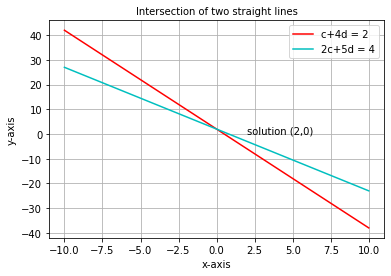
\includegraphics[width=\columnwidth]{plot2.png}
\caption{Plot of the lines}
\label{plt_2}
\end{figure}

Therefore, the matrix $\vec{X}$ is
\begin{align}
  \vec{X} &= \myvec{a & b \\ c & d}\\
          &= \myvec{1 & -2 \\ 2 & 0}
\end{align}

\end{document}

